%!TeX root=../Monografia - Mikhael Pinto.tex
%("dica" para o editor de texto: este arquivo é parte de um documento maior)

% Conteúdo da subseção sobre Contestações
% Este arquivo é importado em 02-implementacao.tex

O algoritmo de validação automática de viagens implementado no backend Flask rejeitava viagens que não atendiam critérios predefinidos: distância < 1km (consideradas muito curtas para deslocamento cotidiano), origem ou destino fora das localizações cadastradas (potencial fraude ou uso recreacional não remunerável), ou trajetória implausível (teletransportes indicando falha de GPS). Embora estes critérios reduzissem tentativas de fraude, geravam falsos positivos: viagem legítima rejeitada por erro temporário de GPS, localização ligeiramente deslocada devido a imprecisão de geocodificação, ou participante que iniciou pedalada próximo mas não exatamente na localização cadastrada. Sistema de contestações oferece canal para reverter rejeições injustas, balanceando a eficiência da automação com a supervisão humana.

No aplicativo móvel, participantes cujas viagens foram reprovadas visualizam botão ``Contestar'' na tela de detalhes da viagem. Ao clicar, preenchem campo de justificativa explicando por que consideram a viagem válida (ex: ``Saí de casa normalmente, mas GPS demorou para conectar'', ``Trabalho fica dentro de prédio comercial, endereço cadastrado é da entrada principal''). A contestação é enviada e cria registro com status pendente de análise, visível imediatamente na interface administrativa.

A tela administrativa de contestações exibe tabela paginada com ID da pessoa, ID da viagem, data, justificativa, e status (Pendente/Sim/Não). Busca textual cobre todos campos, útil para localizar contestações de participante específico (``busca: 123'') ou por palavra-chave na justificativa (``busca: GPS''). Ao clicar em linha, sistema destaca visualmente e carrega detalhes completos abaixo da tabela, incluindo nome do participante, justificativa integral, e mapa interativo renderizando trajeto GPS da viagem contestada. Visualização do trajeto revelou-se decisória: administrador constata se rota realmente conecta origem-destino, se passou por vias cicláveis, ou se apresenta anomalias (ex: linha reta implausível indicando falha de GPS). A visualização dos trajetos será melhor descrita na seção viagens. A Figura~\ref{fig:contestacoes_listagem} mostra a interface de listagem (dados fictícios para fins ilustrativos).

 \begin{figure}[htb]
   \centering
   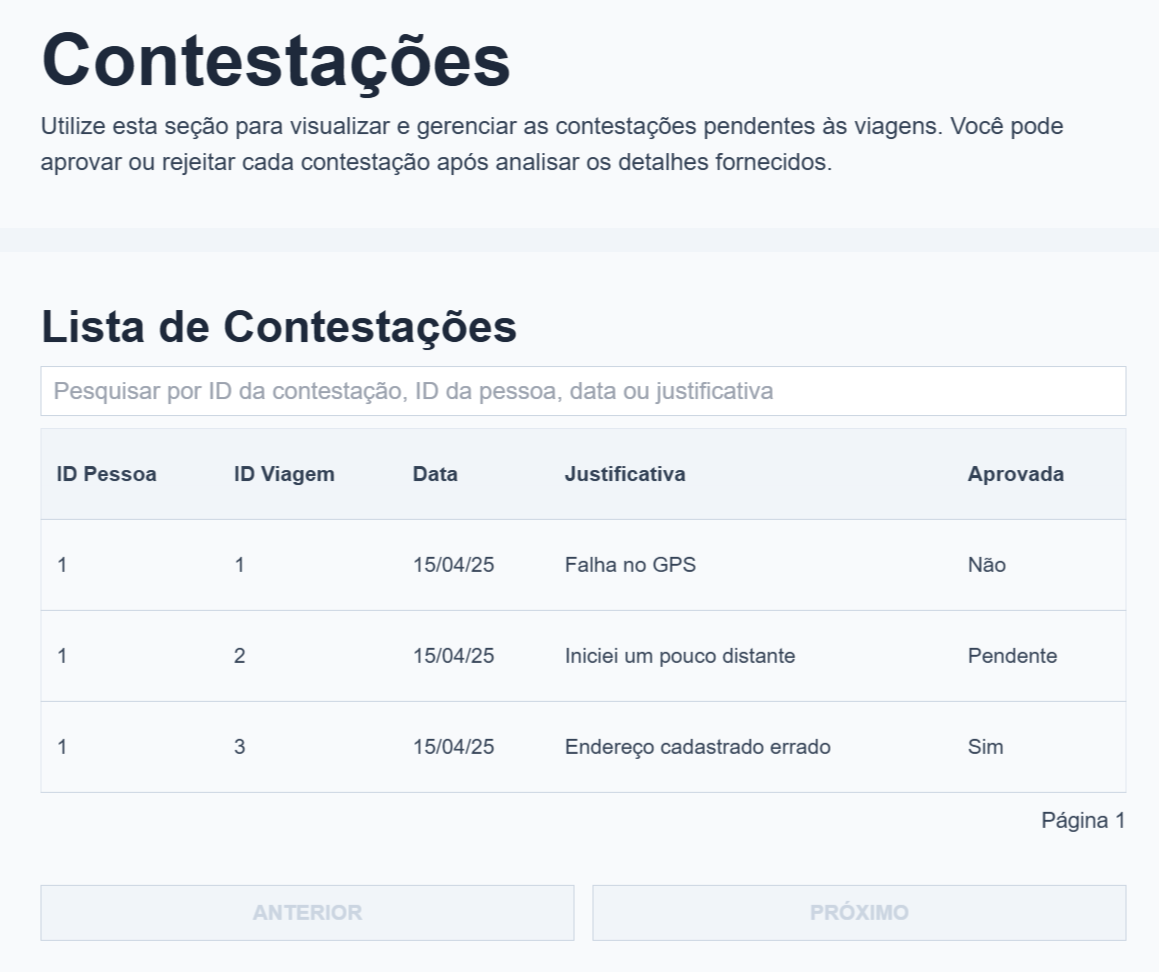
\includegraphics[width=0.95\textwidth]{figuras/contestacoes_listar.png}
   \caption{Interface de listagem de contestações com busca e paginação (dados fictícios).}
   \label{fig:contestacoes_listagem}
 \end{figure}



Após analisar mapa e justificativa, administrador pode aprovar contestação clicando botão com confirmação de duplo clique (prevenção contra aprovação acidental). Sistema executa validações adicionais: contestação não pode ter sido processada anteriormente, viagem deve ter origem e destino definidos e distintos, usuário deve estar em coorte ativa, e distância entre origem-destino $\geq$ 1km. Cálculo de remuneração segue fórmula oficial: \texttt{distancia\_km = min(8000, distancia\_metros) / 1000; remuneracao = distancia\_km * valor\_por\_km\_da\_coorte}. Distância é limitada em 8km (viagens mais longas recebem teto de 8km) para controlar orçamento. Ao aprovar, sistema: atualiza status da viagem para ``Aprovado'', salva valor de remuneração, adiciona crédito à fila de pagamentos, marca a contestação como aprovada, e opcionalmente salva resposta textual do administrador (feedback ao participante). Mensagem de sucesso confirma: ``Contestação da viagem 12345 aprovada com remuneração de R\$ 4,50''. A Figura~\ref{fig:contestacao_aprovar} ilustra a interface de aprovação/rejeição (dados fictícios para fins ilustrativos).

 
\begin{figure}[htb]
    \centering
    
\includegraphics[width=0.95\textwidth]{figuras/contestacao_aprovar.PNG}
    \caption{Interface de aprovação/rejeição de contestação (dados fictícios).}
    \label{fig:contestacao_aprovar}
  \end{figure}

O administrador pode rejeitar contestação (também com confirmação dupla) quando: trajeto não conecta localizações cadastradas (participante tentou viagem recreacional), distância insuficiente mesmo com tolerância, ou justificativa indica má-fé (``não sabia que precisava ativar GPS''). Sistema atualiza contestação para reprovada, salva resposta opcional explicando motivo da rejeição (ex: ``Trajeto iniciou 2km distante da localização cadastrada. Por favor, inicie viagens próximo aos endereços registrados.''), e mantém viagem com status reprovado original. Campo de resposta é exibido no aplicativo móvel, permitindo participante compreender razão e ajustar comportamento futuro.

O sistema implementa múltiplas validações com mensagens específicas orientando correção: ``CONTESTAÇÃO INVÁLIDA'' (ID não encontrado), ``CONTESTAÇÃO JÁ GERENCIADA'' (processamento duplicado prevenido), ``VALOR FALTANDO PARA VIAGEM COM ORIGEM OU DESTINO DESCONHECIDO'' (dados incompletos na viagem), ``VALOR FALTANDO PARA VIAGEM COM ORIGEM == DESTINO'' (mesmo local), ``PESSOA SEM GRUPO PESQUISA'' (usuário não atribuído a coorte), ``DISTANCIA MENOR QUE 1KM'' (critério mínimo não atendido). Estas mensagens, além de prevenir estados inconsistentes no banco de dados, comunicam ao administrador qual condição falhou, permitindo diagnóstico e correção manual (ex: atribuir usuário a coorte antes de reaprovar contestação).
